\documentclass{article}
\usepackage{amsmath, amssymb, geometry}
\usepackage{tikz}
\usepackage{titlesec}
\usepackage{graphicx}
\usepackage{caption}
\usepackage{subcaption}
\usepackage{float}
\usepackage{lmodern}
\usepackage[french]{babel}
\usepackage{hyperref}

\newcommand{\HRule}{\rule{\linewidth}{0.5mm}}
\geometry{a4paper, margin=2.5cm}
\date{\vspace{1cm} \today}

\begin{document}

% Page de titre
\begin{titlepage}
    \centering
    \begin{tikzpicture}[remember picture, overlay]
        \node[opacity=0.1] at (current page.center) {
\includegraphics[width=\paperwidth,height=\paperheight,keepaspectratio]{images/logo.png}};
    \end{tikzpicture}

    \vspace*{2cm}

    {\Huge\bfseries Rapport de modélisation\\[0.5em] \LARGE SAE821 -- Gérer un projet}

    \vspace{1.5cm}

    \HRule
    \vspace{0.5cm}

    \Large{Modélisation UML et architecture du projet}

    \vspace{0.5cm}
    \HRule\\[11cm]

    \begin{flushleft}
        \small
        \textbf{Pegliasco Matteo}\\
        \textbf{Berge Enzo}\\
        \textbf{Audouard Florian}\\
        \textbf{Hermelin Lois}\\
        \textbf{Master Informatique et Mathématiques}\\
        Université de Toulon, La Garde, Var, France
    \end{flushleft}
    \vfill
\end{titlepage}

% ===========================
\section{Introduction}

Ce rapport présente la modélisation UML réalisée dans le cadre du projet. L'objectif est de formaliser le fonctionnement du système à travers des représentations visuelles structurées. 
Cette modélisation permet d'analyser le système sous différents angles fonctionnel, statique et dynamique afin de faciliter sa conception, son développement et sa compréhension par l’ensemble des parties prenantes.

\section{Méthodologie}

Dans le cadre de ce projet, nous avons adopté une démarche rigoureuse de modélisation basée sur les standards UML (Unified Modeling Language). Cette approche nous a permis de représenter de manière structurée et cohérente les différentes facettes du système à développer.

\subsection*{Outils et langages utilisés}
Nous avons utilisé l’outil \textbf{PUML} pour la conception des diagrammes UML.

\subsection*{Démarche de modélisation}
La modélisation a été structurée selon trois axes complémentaires, chacun correspondant à un aspect essentiel du système :

\begin{itemize}
    \item \textbf{Axe Fonctionnel} : Il s'agit de représenter les besoins et les interactions des utilisateurs à travers des \textit{diagrammes de cas d’utilisation} et des \textit{scénarios}.
    
    \item \textbf{Axe Statique} : Cet axe se concentre sur la structure interne du système avec des \textit{diagrammes de classes}, mettant en évidence les entités, leurs attributs, leurs méthodes, ainsi que les relations entre elles (association, agrégation, composition, héritage).
    
    \item \textbf{Axe Dynamique} : Il permet de représenter le comportement du système dans le temps, à l’aide de \textit{diagrammes de séquence}.
\end{itemize}

Cette séparation en trois axes nous a permis d'analyser le système de manière complète et complémentaire, en assurant à la fois une vision fonctionnelle (ce que fait le système), structurelle (comment il est conçu), et comportementale (comment il réagit et évolue).



% ===========================
\section{Histoires Utilisateur}
\subsection{Acteurs identifiés}
\begin{figure}[H]
    \centering
    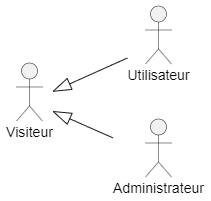
\includegraphics[width=0.35\textwidth]{images/role.png}
    \caption{Diagramme de rôles des acteurs}
\end{figure}
Nous avons identifiés un acteurs général pour notre système de gestion de films, le visiteur, qui peut être un utilisateur ou un administrateur :
\begin{itemize}
    \item \textbf{Visiteur} : peut effectuer des recherches de films, par titre ou genre, et consulter les fiches détaillées des films.
    \item \textbf{Utilisateur} : peut s’inscrire, se connecter, noter les films, laisser des avis.
    \item \textbf{Administrateur} : gère les utilisateurs, gère les avis, gère les films.
\end{itemize}

% ===========================
\section{Modélisation selon l'Axe Fonctionnel}
\subsection{Diagramme de Cas d’Utilisation}
\subsubsection{Le visiteur}
\begin{figure}[H]
    \centering
    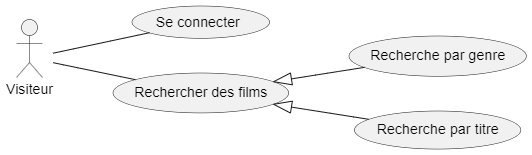
\includegraphics[width=0.5\textwidth]{images/usecase/visiteur.png}
    \caption{Diagramme de cas d’utilisation du visiteur}
\end{figure}
\subparagraph{User Stories}
\begin{itemize}
    \item \textbf{En tant que visiteur}, je peux rechercher des films par titre ou genre.
    \item \textbf{En tant que visiteur}, je peux me connecter.
\end{itemize}
\subsubsection{L'utilisateur}
\begin{figure}[H]
    \centering
    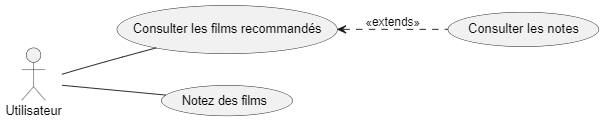
\includegraphics[width=0.5\textwidth]{images/usecase/user.png}
    \caption{Diagramme de cas d’utilisation de l'utilisateur}
\end{figure}
\subparagraph{User Stories}
\begin{itemize}
    \item \textbf{En tant qu'utilisateur}, je peux consulter mes recommandations sans que mes données soient accessibles.
    \item \textbf{En tant qu'utilisateur}, je peux noter les films que j'ai vus sans que mes données soient accessibles.
\end{itemize}
\subsubsection{L'administrateur}
\begin{figure}[H]
    \centering
    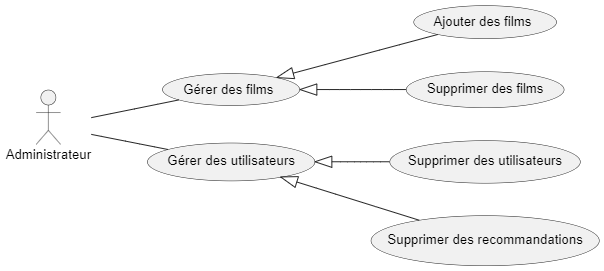
\includegraphics[width=0.5\textwidth]{images/usecase/admin.png}
    \caption{Diagramme de cas d’utilisation de l’administrateur}
\end{figure}
\subparagraph{User Stories}
\begin{itemize}
    \item \textbf{En tant qu'administrateur}, je peux gérer les utilisateurs, les supprimer ou le mettre à jour.
    \item \textbf{En tant qu'administrateur}, je peux gérer les films, les supprimer ou le mettre à jour.
    \item \textbf{En tant qu'administrateur}, je peux gérer les avis, les supprimer ou le mettre à jour.
\end{itemize}

% ===========================
\section{Modélisation selon l'Axe Statique}
\subsection{Diagramme de Classes}
\begin{figure}[H]
    \centering
    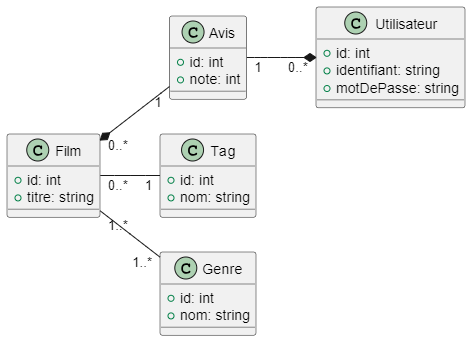
\includegraphics[width=0.5\textwidth]{images/classes/classe.png}
    \caption{Diagramme de classes}
\end{figure}

\subsection{Structure et Relations des Entités}

Le diagramme de classes ci-dessus décrit les entités centrales du système et leurs relations. Voici l’analyse détaillée :

\paragraph{Classes et Attributs}

\begin{itemize}
    \item \textbf{Utilisateur}
    \begin{itemize}
        \item \texttt{id : int} -- Identifiant unique.
        \item \texttt{identifiant : string} -- Nom d'utilisateur.
        \item \texttt{motDePasse : string} -- Mot de passe de connexion.
    \end{itemize}
    
    \item \textbf{Avis}
    \begin{itemize}
        \item \texttt{id : int} -- Identifiant unique.
        \item \texttt{note : int} -- Note donnée par l'utilisateur pour un film.
    \end{itemize}

    \item \textbf{Film}
    \begin{itemize}
        \item \texttt{id : int} -- Identifiant unique.
        \item \texttt{titre : string} -- Titre du film.
    \end{itemize}

    \item \textbf{Tag}
    \begin{itemize}
        \item \texttt{id : int} -- Identifiant unique.
        \item \texttt{nom : string} -- Nom du tag.
    \end{itemize}

    \item \textbf{Genre}
    \begin{itemize}
        \item \texttt{id : int} -- Identifiant unique.
        \item \texttt{nom : string} -- Libellé du genre.
    \end{itemize}
\end{itemize}

\paragraph{Relations entre les classes}

\begin{itemize}
    \item \textbf{Utilisateur -- Avis : Composition (1 à 0..*)}
    \begin{itemize}
        \item Un utilisateur peut rédiger plusieurs avis.
        \item Un avis appartient obligatoirement à un utilisateur.
        \item Il s’agit d’une \textbf{composition}, car un avis ne peut pas exister sans l’utilisateur qui l’a créé.
    \end{itemize}

    \item \textbf{Film -- Avis : Composition (1 à 0..*)}
    \begin{itemize}
        \item Un film peut avoir plusieurs avis.
        \item Chaque avis est lié à un seul film.
        \item C’est aussi une \textbf{composition}, car un avis n’a de sens que s’il est associé à un film.
    \end{itemize}

    \item \textbf{Film -- Tag : Association (0..* à 0..1)}
    \begin{itemize}
        \item Un film peut être associé à plusieurs tags.
        \item Chaque tag est associé à un seul film.
        \item Cela restreint la réutilisabilité d’un tag ; une association \textbf{n-n} serait plus cohérente dans une optique réaliste.
    \end{itemize}

    \item \textbf{Film -- Genre : Association (1..* à 1..*)}
    \begin{itemize}
        \item Un film doit être classé dans au moins un genre.
        \item Un genre peut s’appliquer à plusieurs films.
    \end{itemize}
\end{itemize}

% ===========================
\section{Modélisation selon l'Axe Dynamique}
\subsection{Diagramme de Séquence}
\subsubsection{L'utilisateur}
\begin{figure}[H]
    \centering
    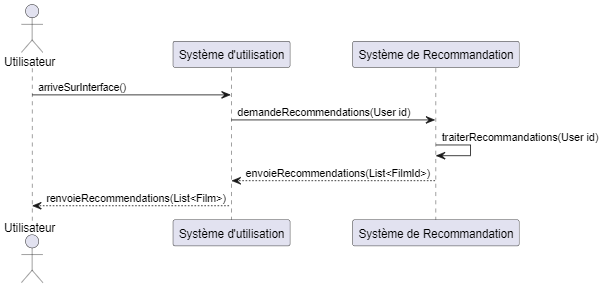
\includegraphics[width=0.9\textwidth]{images/sequence/user/seq_user_1.png}
    \caption{L'utilisateur consulte ses recommandations}
\end{figure}
\begin{figure}[H]
    \centering
    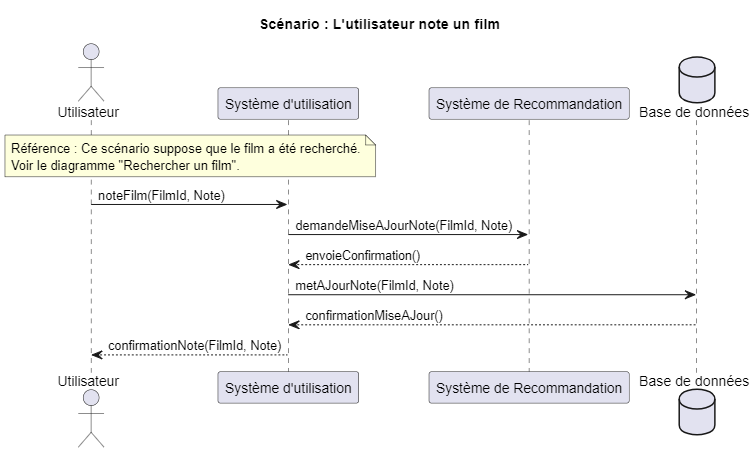
\includegraphics[width=0.9\textwidth]{images/sequence/user/seq_user_2.png}
    \caption{L'utilisateur note un film}
\end{figure}
\begin{figure}[H]
    \centering
    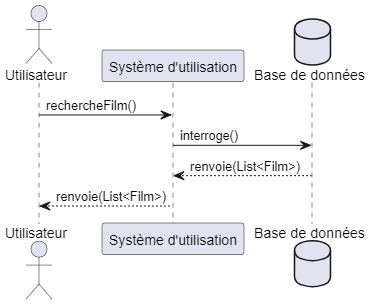
\includegraphics[width=0.5\textwidth]{images/sequence/user/seq_user_3.png}
    \caption{L'utilisateur recherche un film}
\end{figure}

\subsubsection{L'administrateur}
\begin{figure}[H]
    \centering
    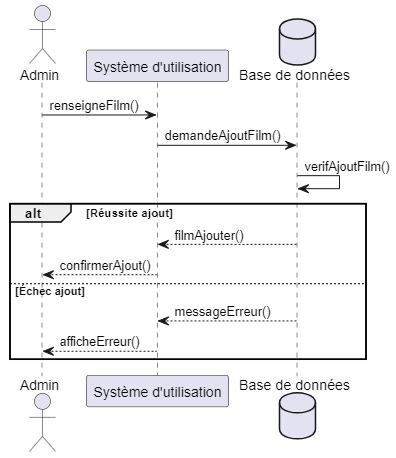
\includegraphics[width=0.6\textwidth]{images/sequence/admin/seq_admin_1.png}
    \caption{L'administrateur ajoute un film}
\end{figure}
\begin{figure}[H]
    \centering
    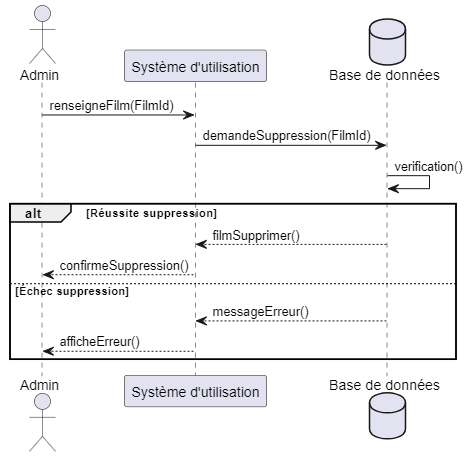
\includegraphics[width=0.6\textwidth]{images/sequence/admin/seq_admin_2.png}
    \caption{L'administrateur supprime un film}
\end{figure}
\begin{figure}[H]
    \centering
    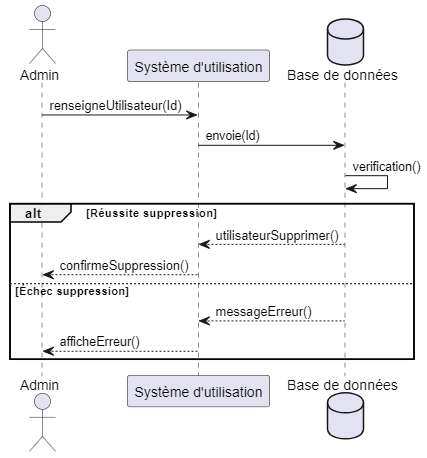
\includegraphics[width=0.6\textwidth]{images/sequence/admin/seq_admin_3.png}
    \caption{L'administrateur supprime un utilisateur}
\end{figure}

% ===========================
\section{Analyse Complémentaire}
\subsection{Diagramme de Déploiement}
\begin{figure}[H]
    \centering
    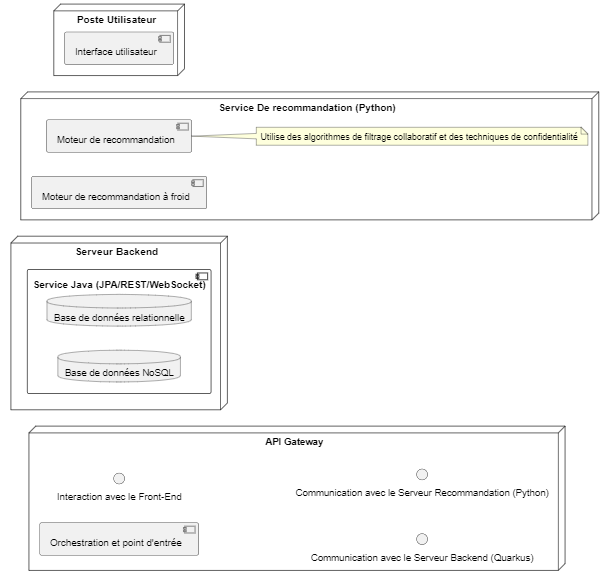
\includegraphics[width=0.75\textwidth]{images/deploiement/deploiement.png}
    \caption{Diagramme de déploiement du système}
\end{figure}

% ===========================
\section{Conclusion}

L’ensemble de cette modélisation offre une base solide pour la conception, le développement et l’évolution du système. Elle assure une meilleure compréhension commune entre les membres de l'équipe projet, facilite la documentation et peut également servir de support à la validation fonctionnelle auprès du client ou des utilisateurs.

Les choix de représentation ont été faits pour maximiser la clarté, tout en restant fidèles aux exigences initiales du projet. Bien que certaines parties restent simplifiées ou perfectibles, la cohérence globale du modèle a été maintenue.




\end{document}
